% Some commands used in this file
\newcommand{\product}{\textit}

\chapter{Material and Methods}

\section{General information}
All the liquids that contact the cell, were pre-warmed in a water-bath to limit cold-exposure. Unless stated otherwise, we worked under sterile conditions. By courtesy of Prof. Ivan Martin (University of Basel), we had access to human bone-marrow derived mesenchymal stem cells from pseudonymized patients. Incubation parameters are kept constant at 37 \degC and 5\% CO\textsubscript{2} in humidified air. Light microscopy pictures of cells are taken using an EVOS inverted light micrscope (ThermoFisher).

\section{Statistical Analysis}
We either used Windows Excel or GraphPad Prism v8 for statistical analysis. The chosen test metric is indicated in every figure legend.

\section{Cell Culture and Passaging}
Cells are grown in growth medium under sterile conditions. Nunc\texttrademark{} EasYFlask\texttrademark{} Cell Culture Flasks with filters (ThermoFisher) were used for growing the cells. The media was changed every three days. Passaging was done at 80\% confluence using the following standard TE-protocol. First, the cells are washed with PBS. Second, 2ml Trypsin-EDTA (TE, maduzi) is added and the cells incubated for 3-10 minutes. Then, add 10ml MEM\textalpha{} with 10\% FBS and transfer cell solution to 15ml Falcon Tube. Centrifuge for 5 minutes at a speed of 500 rcf. Next, discard the supernatant and resuspend the cells in Growth Medium and seed according to application with typical seeding density being 10\textsuperscript{6} Cells / 75 cm\textsuperscript{2}. 
Growth Medium consist of ROTI\textregistered{} Cell Eagle's MEM\textalpha{} with nucleosides and stable l-glutamine(ROTH), 10\% FBS (heat-inactivated, ThermoFisher) and 5ng/ml Growth Factor FGF-2 (PeproTech).

\section{Retroviral Transduction}
\label{sec:RetroVir}
From 100\% confluent MSCs, three T25 flasks (Sigma-Aldrich) were seeded with 800'000 cells according to standard protocol. On the next day, the medium was removed and 1ml of Polybrene Medium (MEM\textalpha{}, 5\% FBS, 1\mul{}/ml Polybrene (Sigma-Aldrich)) added. From here onward, Biosafety Level (BL) 2 measures were applied. Carefully, 1ml of virus construct was added to corresponding flask and incubated at 4 \degC for 2 hours. This was then followed by addition of 3ml Compensation-Medium (3ml MEM\textalpha{}, 5\% FBS, 1\mul{}/ml Polybrene and 8 ng/ml FGF-2), after which the cells were incubated over night. On the next day, the medium was removed and 5ml standard Growth Medium added. On the next day, the cells were split 1:3.5 depending on confluence. On the day after, selection was started by removing old medium and adding Selection Medium (Growth Medium + 3\textmu{}g/ml Puromycin (Thermo Fisher Scientific)) and incubating the cells for 72 hours. After selection phase ended we exchanged the medium with Growth Medium. Then over the next 5-6 days, the media of the cells was changed another three times until the virus particles are neutralized and the BL restrictions can be relaxed from BL2 to BL1. Efficiency of knock-out is  assessed with Western Blot (Protein) and qRT-PCR (mRNA). Then the cells are either frozen or seeded according to need. 

Three different viral constructs were used (2 distinct \Piezo{} knock-out and one negative control, one per flask) using pre-made lentivirus, carrying a specific CRISPR/Cas9-system with puromycin resistance as the selection marker. The knock-out is defined through the construct used, resulting in cell lines P1-395, P1-555 and NoT. P1-395 describes the cell line with base deletion in \PiezoGene{}-gene at position 395, similarly P1-555 describes deletion at position 555 and NoT describes control for viral transduction with no putative mutation in genome.


\section{RNA Analysis}
\subsection{RNA Extraction}
This was prepared in open space. Cells were either directly lysed in-well after PBS washing or lysed in the tube, after being collected from well and washed with PBS. Lysis-Buffer was supplemented with 1\% \textbeta-mercaptoethanol. The whole cell lysate was either frozen for later processing or directly processed. When freezing the lysate, the tube is shock-frozen in liquid nitrogen before transferred to -80 \degC freezer. When processing, the PureLink PCR Micro Kit (\product{Thermo Fisher, CN: K310250}) following manufacturer's protocol was used, dissolving the RNA in the final step with 20\mul{} of RNase-free Water (BioConcept). The final concentration of the sample was assessed using the Qubit RNA HS Assay Kit (ThermoFisher) with a new calibration each time a new working solution was prepared.

\subsection{Reverse Transcription}
This was prepared in open space. Unless stated otherwise, 300ng of RNA was transcribed per 40\mul{} total reaction volume using the High-Capacity cDNA Reverse Transcription Kit (Thermo Fischer) following supplier's instructions to produce cDNA. The samples were kept at 37 \degC for 2 hours followed by 5 min at 95 \degC with the thermal Mastercycler (Eppendorf) to terminate the generation of cDNA. Samples were either stored at -20 \degC or used directly. 

\subsection{Quantitative Real-Time PCR Analysis}
All real-time PCR analyses were performed on a StepOnePlus ThermoCycler real-time PCR system (Applied Biosystems) with a 96-well plate as a carrier device. Each reaction well contained a reaction volume of 2\mul{} sample cDNA and 8\mul{} Primer-specific PCR MasterMix (KAPA PROBE FAST MasterMix (KAPA Biosystems), TaqMan\textregistered{} Primer (ThermoFisher) and RNase-free Water). The cDNA was amplified using the following protocol: First, a denaturating stage where samples were kept at 95 \degC for 10
min, followed by an annealing stage that consisted of 40 cycles of 95 \degC for 10sec and extending stage at 60 \degC for 30sec. All samples were run in technical triplicates. The C\textsubscript{t}-value (cycle threshold) value for each gene was determined using the automated threshold analysis in the StepOnePlus device. Data was evaluated using the comparative C\textsubscript{t}-Method with GAPDH and RPL13A as housekeeping genes.

Investigated gene products and corresponding primers used are (Product Number TBA): 

\begin{tabular}{lr}
	Gene & Number \\ 
	\hline 
	\rule[-1ex]{0pt}{4ex}  &  \\ 
	\textit{COL1A1} & Hs00164004\_m1 \\ 
	\hline 
	\rule[-1ex]{0pt}{2.5ex}  &  \\ 
	\textit{COL3A1} & Hs009443809\_m1 \\ 
	\hline 
	\rule[-1ex]{0pt}{2.5ex}  &  \\ 
	\textit{FN1} & Hs01549976\_m1 \\ 
	\hline 
	\rule[-1ex]{0pt}{2.5ex}  &  \\ 
	\textit{IL-6} & Hs00174131\_m1 \\ 
	\hline 
	\rule[-1ex]{0pt}{2.5ex}  &  \\ 
	\textit{ALPL} & Hs01029144\_m1 \\ 
	\hline 
	\rule[-1ex]{0pt}{2.5ex}  &  \\ 
	\textit{RUNX2} & Hs00231692\_m1 \\ 
	\hline 
	\rule[-1ex]{0pt}{2.5ex}  &  \\ 
	\textit{SPP1} & Hs00959010\_m1 \\ 
	\hline 
	\rule[-1ex]{0pt}{2.5ex}  &  \\ 
	\textit{GAPDH} & Hs02758991\_g1 \\ 
	\hline 
	\rule[-1ex]{0pt}{2.5ex}  &  \\ 
	\textit{RPL13A} & Hs04194366\_g1 \\ 
\end{tabular} 


\section{Protein Analysis}
\subsection{Preparation}
After washing the cells with PBS, 0.5ml of TE(1X) was added to each well, after which the cells where incubated for 3-8 minutes. As to maximize yield, we additionally employed a scraping protocol. 1ml of MEM\textalpha{} + 10\% FBS is added per well and the cells gently scraped off using a cell scraper (16cm, Sarstedt). Then transfer the cells into an eppendorf tube, followed by a RT centrifugation step at 2'000 rcf for 5 minutes after which the supernatant is discarded. Then the tube is filled with 1.5ml of PBS and the centrifugation step including the discarding of supernatant repeated. Finally, the tubes are shock-frozen in liquid nitrogen before transferring them to a -80 \degC freezer for storage. When processing, the protein samples, the whole cell pellet was dissolved in 20\mul{} of \textsc{Ripa}-Buffer (Sigma-Aldrich). After incubation on ice for 20 minutes, during which each sample was vortexed three to four times, the samples are 4 \degC centrifuged at maximum speed for 10 minutes. For further processing, only the supernatant is used. Measure protein concentration of all samples by employing the DC\texttrademark{} Protein Assay (BioRad), following the manufacturer's protocol and comparing it to a standard curve. Then protein concentration was normalized while maximized (i.e. dilute with RIPA all samples to match concentration of lowest concentration sample). \\
The standard curve has been generated once by preparing multiple dilutions of a Bovine Serum Albumine standard with a known concentration of 2mg/ml (BioRad) with \textsc{Ripa}-Buffer. The dilutions, having concentrations of 0mg/ml, 0.25mg/ml, 0.5mg/ml, 0.75mg/ml, 1mg/ml, 1.5mg/ml and 2mg/ml BSA, were then measured in triplicates the adsorption (\textlambda{} = 750nm) following the manufacturers standard procotol. The average of triplicates was calculated and a standard curve fitted to the data points that relates signal to protein-concentration. 

\subsection{Western Blotting}
In new tube Laemmli-Buffer(6X) (BioRad) and sample was mixed to a final volume of 15\mul{} (protein content per lane was normalized over a blot, protein loaded varied between blots from 3.64 to 5.8 \textmu{}g), then  vortexed 5 seconds and then cooked for 4-8 minutes at 95 \degC in ThermoCycler (i.e. cooking), where each tube contained the same amount of protein. Then the sample was loaded onto a 4–15\% Mini-PROTEAN TGX Stain-Free Protein Gel (BioRad) and resolved by electropphoresis at constant current of 35mA. Then the gel is wet-transferred onto PVDF Membrane (BioRad) using Trans-Blot Turbo Transfer System (BioRad) with settings either High MW (1.3 A, 25V, 10min) for blot in Fig.~\vref{fig:KO-Verification}, and Mixed MW (1.3A, 25V, 7min) for the remaining. The membrane was then blocked in 5 wt\% low fat dry-milk (Migros) in TBST (i.e. blocking solution) for 1 hour. This is followed by shaken incubation primary antibody either for 2 hours at room temperature or 14 hours at 4 \degC{}. After 3 times 10min washing in TBST, the membrane is incubated in the matching secondary antibody, which is conjugated to HRP. Every time before immersion medium changes, the membrane was washed three times in TBST for 10 minutes. SuperSignal Ultra/Femto detection reagents (Pierce) were used for visualization (Femto for blot in Fig.~\vref{fig:KO-Verification}, Ultra for the remaining). The exposure time were manually set to accommodate maximum signal while avoiding saturation. Only after successful imaging of the protein of interest, incubation with primary housekeeping protein antibody was started. Quantification was done manually with Fiji (version 2.0.0-rc-69, Java 1.8) with the analysis workflow described elsewhere \cite{Miller2010}.



\begin{itemize}
    \item Primary Antibodies
    \begin{itemize}
		\item[COL1A1] rabbit Collagen I antibody (GTX112731, Genetex) in 5wt\% BSA (lyophilized, VWR)in TBST, 1:2'000
		\item[\PiezoGene{}] rabbit Anti-PIEZO1 antibody (NBP1-78446, Novus) in 5wt\% BSA (lyophilized) in TBST, 1:1'000
		\item[\textalpha{}-Tub] mouse Anti-alpha-Tubulin (SC-23948, Santa Cruz Biotechn. Inc.) in OneStep Blocker (Lucerna Chem AG) , 1:3'500
		\item[\FnGene{}] rabbit Anti-Fibronectin antibody (F3648, MilliporeSigma) in 4wt\% BSA (lyophilized) in TBST, 1:2'000 F3648-100UL
		\item[\colthreeGene{}] rabbit Anti-Collagen III antibody (ab7778, Abcam) in 5wt\% BSA (lyophilized) in TBST, 1:2'000
    \end{itemize}

 	\item Secondary Antibodies
    \begin{itemize}
		\item[anti-mouse] goat anti-mouse with conjugated HRP (SAB3701073, Sigma-Aldrich) in 2.5wt\% low-fat dry milk in TBST 
		\item[anti-rabbit] goat anti-rabbit with conjugated HRP (SAB3700878, Sigma-Aldrich) in 2.5wt\% low-fat dry milk in TBST 
    \end{itemize}
\end{itemize}


\section{Chemical stimulation of \Piezo{} with \Yoda{}}
\label{sec:ChemicalStimulation}
At any timepoint during this whole experiment cells are kept serum starved and without supplementation of FGF-2.\\
Confluent cells were seeded serum-starved on 6 well plates at concentration of 240'000 cells/well and incubated for 8-14 hours.\\
The intervention is then initiated with a washing step, before 2.5ml of Intervention Medium (i.e. MEM\textalpha{} + 5\textmu{}M \Yoda (Sigma-Aldrich), concentration defined as suggested by Morley et al. \cite{Morley2018}.) is added. Negative control samples were supplemented with MEM\textalpha{} only. The cells were then incubated under standard conditions for 30 minutes, after which they are washed twice, before adding MEM\textalpha{} as culture medium and incubating cells until harvesting. RNA and Protein samples were collected using the respective standard protocol.\\ as for evidence for correct concentration. Unless specified otherwise, \Yoda{}-intervention consisted of cells being exposed to MEM\textalpha{} supplemented with 5\mul{}M \Yoda{} for 30 minutes. 

\section{Fluidic Shear Stress Setup}
As the result of the Masters Thesis Project from Patrick Jäger, we have access to flow chambers, which describes a type of platform that allows us to apply fluidic shear stress to cells in a fully controlled environment. This flow chamber allows arbitrary choice of shear media, cell type and cellular alignment relative to flow, while leaving the researcher the opportunity to choose from either in-situ real-time calcium imaging, re-cultivation for additional steps or direct downstream processing.

\subsection{Flow chamber and seeding}
\label{sec:FluidicModel}
To fabricate the PDMS part of the flow chamber, firstly, 10 parts of silicone (SYLGARD\texttrademark{} 184 Elastomer Base Component, Dow) and 1 part of cross-linker (SYLGARD\texttrademark{} 184 Elastomer Curing Component, Dow) are combined and vigorously mixed for 5 minutes using a single-use spatula. Then put in vacuum chamber that oscillates between 60 and 120 mbar to allow enclosed air to leave the gel. Put the gel in negative, metal form, then vacuum again. The form is then put on heating plate over-night at 70 \degC{}. After the microscopy slides underwent plasma treatment for 4 minutes, we glue a stamp on the slide using the silicon-crosslinker-mixture from earlier. Then we put them over night next to the metal form on a heating plate. On the next day, remove the PDMS stamps from microscopy slide, leaving behind PDMS grating. Decorate the stamps with Rat Tail Collagen-1 (3.47mg/ml, Corning) using Sulfo-SANPAH (ProteoChem) as a crosslinker. Proceed with separating the flow chamber pieces and punch entry point of 4mm diameter as access point for syringe system. Prepare glue by adding 3\mul of Platinum reagent (Platinum-Divinyltetramethyldisiloxan complex in Xylene, Gelest) to 1g of silicon, then mix for 3 minutes. Add 0.1g of Crosslinker, mix again for 5 minutes. Now glue PDMS-pieces on glass slide and put in oven at 45 \degC{} for 2 hours. Either we stored them in the fridge or seed cells for an experiment on the next day.\\
For seeding, we work sterile in the cell culture lab. Flow chambers are sterilised using 80\% EtOH (including flushing of chamber) and kept in fume hood until air-dried. Flush the chamber twice with PBS. Prepare cell solution of 10\textsuperscript{6} MSCs/ml in Growth Medium. Add 70 \mul{} of cell solution per flow chamber and incubate the chambers for 45 minutes. Then, flush the chamber with 200\mul{} of Growth Medium to remove non-adherent cells, while making sure to avoid cell-air contact. Put in incubator over night with the experiment scheduled on the next day.\\

In preparation for an experiment on the next day we prepared shear media, which is either normal, \calcium{}-containing artificial cerebrospinal fluid (ASCF) or \calcium{}-free ACSF. For each ACSF solution to be prepared we took a 0.5l Duran Bottle. For normal ACSF we added 0.9g of Glucose and 0.11g of CaCl\textsubscript{2} to the bottle. For \calcium{}-free ACSF we added 0.9g Glucose, 0.095g MgCl\textsubscript{2} and 0.38g EGTA. Then we added to each bottle 250ml of Stock Solution A and 250ml of Stock Solution B. Then we bubbled the solution for more than 15min with N\textsubscript{2} and CO\textsubscript{2} to allow for dissolving. After bubbling is finished we ultra-filtrated the solution in a sterile Duran Bottle under sterile conditions and transferred it to the incubator, with the top loosely closed, where we leave it over-night.

\subsection{Fluorescence staining and imaging}
\label{sec:LiveImaging}




\begin{figure}
	\centering
	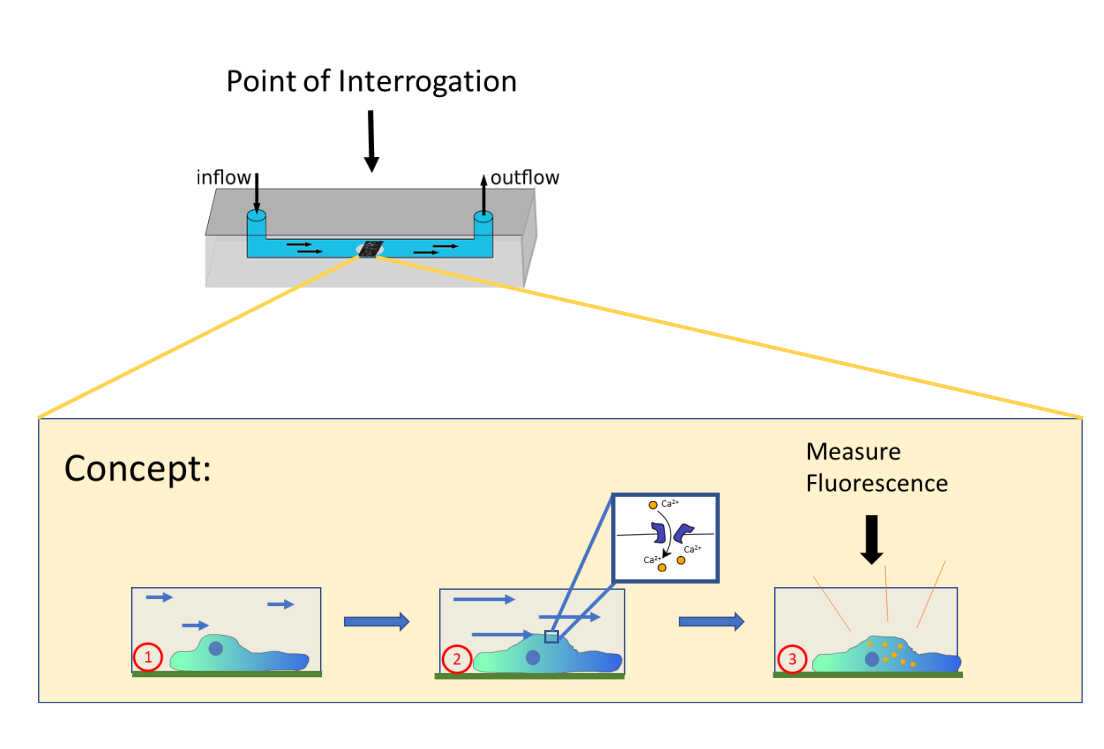
\includegraphics[width = 0.8\textwidth]{FlowChamberSchematic.png}
	\caption{Schematic depiction of physical setup (top) and conceptual workflow (bottom) of live calcium imaging in this shear stress setup.}
	\label{fig:FlowChamberSchematic}
\end{figure}


On the day of the experiment, we pre-incubated sufficient Growth Medium for more than 30min under standard conditions. In 500\mul{} of pre-incubated Growth Medium we added 2\mul{} of Fluo-4 (1mM, ThermoFisher) (i.e. Staining Medium). Then we added 200\mul{} of Staining Medium to each flow chamber and incubated them at standard conditions for 2h until the start of the experiment. Before the experiment, we prepared the syringe system (Cetoni), filling the syringes with corresponding shear media and pre-configuring the shear flow-protocol. Also we prepared the microscope and pre-configured the imaging protocol. Imaging protocol was configured in LiveAcquisition (v1.2.2, TILL Photonics) with duration of 120s per measurement incorporating a Z-stack of five pictures per second to account for shear-mediated displacement of cell.
After incubation of flow chambers with Staining Medium ended, we connected the syringe with the inlet on the flowchamber and an outlet to a flask for extruded media. Before the start of the experiment, we flushed the flowchamber with media for 10min with a flowrate of 0.2ml/min. Then manually trigger simultaneously the execution of both imaging and shear-flow protocol.\\
If a second measurement with the same flowchamber was scheduled, we flushed the flowchamber for 12min with 2.4ml with exchanged media before triggering a second measurement.\\
After the measurements, we made a Z-stack projection using the average intensity method.\\
The sequence of first \calcium{}-free and second normal medium is important, as reactive capability of the cells has to be demonstrated in the last measurement to rule out cell death as a possible explanation for lack of impulse response.\\
The shear flow protocol we used consisted of 0.1 ml/min for 30s, then 7 ml/min (equivalent to 7Pa) for 5s, then 0.1ml/min for the remainder of the measurement. 

\subsection{Processing and evaluation}
\label{sub:Processing}

The time-trace of brightness levels of individually segmented cells was done using a workflow implemented in R and ImageJ scripts by Patrick Jäger, using ImageJ (v1.52p) and R Studio. Simplified the workflow consisted of following steps:

\begin{itemize}
	\item Segmentation of cells using the first frame, feeding them in the ROI Manager
	\item Record brightness levels over the whole measurement
	\item Normalization of each brightness for each cell individually using the average of first 15 frames (Leading to one table per flow chamber with size Frames$\times$Cells)
	\item Pooled data of all flow chambers belonging to the same patient in one table
	\item Reduce to matrix of size Frames$\times$3, with columns being Cell Count, Average Signal and Standard Deviation
	\item Maximum Value was found using maxVal-Function over the whole measurement interval
\end{itemize}

Important details are that per recording there was exactly one normalization, leading to seemingly discontinuous jumps in the concatenated measurements of changing flushing medium. Also, we did not manually adjust ROIs. 



